% Comment lines start with %
% LaTeX commands start with \
% This template was provided by Jennifer Welch for CSCE 222-200, Honors, Spring 2015

\documentclass[12pt]{article}  % This is an article with font size 12-point

% Packages add features
\usepackage{times}     % font choice
\usepackage{amsmath}   % American Mathematical Association math formatting
\usepackage{amsthm}    % nice formatting of theorems
\usepackage{amssymb}
\usepackage{amsfonts}
\usepackage{latexsym}  % provides some more symbols
\usepackage{fullpage}  % uses most of the page (1-inch margins)
\usepackage{tikz}
\usepackage{graphicx}

\setlength{\parskip}{.1in}  % increase the space between paragraphs

\renewcommand{\baselinestretch}{1.1}  % increase the space between lines

% Convenient renaming of symbols for logic formulas
\newcommand{\NOT}{\neg}
\newcommand{\AND}{\wedge}
\newcommand{\OR}{\vee}
\newcommand{\XOR}{\oplus}
\newcommand{\IMPLIES}{\rightarrow}
\newcommand{\IFF}{\leftrightarrow}

% Actual content starts here.
\begin{document}

\begin{center}         % center all the material between begin and end
{\large                % use larger font
CSCE 222 (Carlisle), Discrete Structures for Computing \\  % \\ is line break
Spring 2022 \\
Homework 3}
\end{center}
\rule{6in}{.1pt}       % horizontal line 6 inches long and .1 point high
\begin{center}
{\large
Type your name below the pledge to sign\\
On my honor, as an Aggie, I have neither given nor received unauthorized aid on this academic work.\\
**YOUR NAME HERE**}
\end{center}

% blank line separates paragraphs.  First line of a paragraph is automatically
% indented.  

\rule{6in}{.1pt}       % horizontal line 6 inches long and .1 point high
                    
\noindent              % don't indent
{\bf Instructions:}    % \bf makes text boldface
                       % \em makes text emphasized (italics)

\begin{itemize}        % makes an itemized list
\item The exercises are from the textbook.  You are encouraged to work
      extra problems to aid in your learning; remember, the solutions to 
      the odd-numbered problems are in the back of the book.
\item Grading will be based on correctness, clarity, and whether your
      solution is of the appropriate length.
\item Always justify your answers.
\item Don't forget to acknowledge all sources of assistance in the section below, and write up your solutions on your own.
\item {\em Turn in .pdf file to Gradescope by the start of class on Monday February 7, 2022.}  It is simpler to put each problem on its own page using the LaTeX clearpage command.
\end{itemize}


\rule{6in}{.1pt}       % horizontal line 6 inches long and .1 point high

{\bf Help Received:}    % \bf makes text boldface
\begin{itemize}
\item List any help received here, or "NONE".
\end{itemize}



\rule{6in}{.1pt}       % horizontal line 6 inches long and .1 point high

%---------------------------------------------------------------------

% \subsection makes a subsection heading; * leaves it unnumbered.
% (Usually subsections are inside sections, but the \section command
% used a font that was larger than I wanted.)

%--------------------------------------------------------------------





%--------------------------------------------------------------------

\subsection*{Exercises for Section 1.8:}     

\noindent{\bf{8: (2 points)}}\newline
\noindent{Prove using the notion of without loss of generality that $5x+5y$ is an odd integer when $x$ and $y$ are integers of opposite parity.}\newline
\newline
Without loss of generality,\newline
Let $x=2a, a\in\mathbb{Z}$\newline
Let $y=2b+1, b\in\mathbb{Z}$\newline

\noindent{$5x+5y=5(2a)+5(2b+1)$\newline
$=10a+10b+5=2(5a+5b+2)+1$}\newline
$2(5a+5b+2)+1$ is odd.\newline
$\blacksquare$

\noindent{\bf{20: (2 points)}}
\newline
\noindent{Show that if $r$ is an irrational number, there is a unique integer $n$ such that the distance between $r$ and $n$ is less than $\frac{1}{2}$.}\newline
\newline
Let $n\in\mathbb{Z}, m\in\mathbb{Z}, |n-m|\geq1$\newline
With this, suppose that $(|r-n|<\frac{1}{2})\AND(|r-m|<\frac{1}{2})$.\newline
From this, $|n-m|\leq|r-n|+|r-m|<\frac{1}{2}+\frac{1}{2}=1$.\newline
This forces $|n-m|<1$. However this contradicts with the fact that $|n-m|\geq1$.\newline
Because of this only one integer $n$ can exist such that the distance between $r$ and $n$ is less than $\frac{1}{2}$.
$\blacksquare$

\clearpage

\noindent{\bf{32: (2 points)}}\newline
\noindent{Prove that there are no solutions in integers $x$ and $y$ to the equation $2x^2+5y^2=14$.}\newline
Let $x\in\mathbb{Z},y\in\mathbb{Z}$\newline
With this, $x^2\geq0\AND y^2\geq0$.\newline
If $y\leq-2\OR y\geq2$, then $y^2\geq4$ and $5y^2\geq20$. However $5y^2\geq20$ is a contradiction. This forces that $y=-1,y=0,y=1$. We can look at each of these cases separately.\newline
\newline
When $y=-1\OR y=1$; then $2x^2=9$; the left-hand side is even, when the right-hand side is odd. This equation has no integer solution.\newline
\newline
When $y=0$ then $2x^2=14$ or $x^2=7$. We can check all possible values of $x$.
\begin{itemize}
    \item $x=0$; then $x^2=0\neq7$
    \item $x=\pm1$; then $x^2=1\neq7$
    \item $x=\pm2$; then $x^2=4\neq7$
    \item $|x|\geq3$; then $x^2\geq9>7$
\end{itemize}

\noindent{With these cases, there are no integers $x$ and $y$ that satisfy the equation $2x^2+5y^2=14$}\newline
$\blacksquare$

\clearpage

\subsection*{Exercises for Section 2.1:}     

\noindent{\bf{24: (2 points). (Prove your answer is correct.)}}\newline
\noindent{Can you conclude that $A=B$ if $A$ and $B$ are two sets with the same power set?}\newline
Assume $A\neq B$.\newline
$x\in A, x\not\in B$\newline
Because of this $\{x\}\in\mathcal{P}(A), {x}\not\in\mathcal{P}(B)$\newline
However, this contradicts with the fact that $\mathcal{P}(A)=\mathcal{P}(B)$ which must contain the same elements.\newline
$\blacksquare$
\newline

\noindent{\bf{34(a-d): (2 points)}}\newline
\noindent{Let $A=\{a,b,c\}$, $B=\{x,y\}$, and $C=\{0,1\}$. Find}
\begin{enumerate}
    \item $A\times B\times C$\newline
        $\{(a,x,0),(a,x,1),(a,y,0),(a,y,1),$\newline
        $(b,x,0),(b,x,1),(b,y,0),(b,y,1),$\newline
        $(c,x,0),(c,x,1),(c,y,0),(c,y,1)\}$
        
    \item $C\times B\times A$\newline
        $\{(0,x,a),(0,x,b),(0,x,c),(0,y,a),(0,y,b),(0,y,c),$\newline
        $(1,x,a),(1,x,b),(1,x,c),(1,y,a),(1,y,b),(1,y,c)\}$
    \item $C\times A\times B$\newline
        $\{(0,a,x),(0,a,y),(0,b,x),(0,b,y),(0,c,x),(0,c,y),$\newline
        $(1,a,x),(1,a,y),(1,b,x),(1,b,y),(1,c,x),(1,c,y)\}$
    \item $B\times B\times B$\newline
        $\{(x,x,x),(x,x,y),(x,y,x),(x,y,y),(y,x,x),(y,x,y),(y,y,x),(y,y,y)\}$
\end{enumerate}

\clearpage

\noindent{\bf{46(a-d): (2 points)}}\newline
\noindent{Translate each of these quantifications into English and determine its truth value.}
\begin{enumerate}
    \item $\exists x\in\mathbb{R}(x^3=-1)$\newline
        There exists a real number $x$ whose cube is $-1$.\newline
        True $x=-1$
    \item $\exists x\in\mathbb{Z}(x+1)>x$\newline
        There exists an integer $x$ such that $x+1$ is greater than $x$.\newline
        True $x=0$
    \item $\forall x\in\mathbb{Z}(x-1\in\mathbb{Z})$\newline
        For all integers $x$, $x-1$ is also an integer.\newline
        True\newline
        Let $f(x)=x-1$.\newline
        $f:\mathbb{Z}\IMPLIES\mathbb{Z}$
    \item $\forall x\in\mathbb{Z}(x^2\in\mathbb{Z})$\newline
        For all integers $x$, $x^2$ is also an integer.\newline
        Let $f(x)=x^2$\newline
        $f:\mathbb{Z}\IMPLIES\mathbb{Z}$
\end{enumerate}
\clearpage
%--------------------------------------------------------------------

\subsection*{Exercises for Section 2.2:}     

\noindent{\bf{14: (2 points)}}\newline
\noindent{Find the sets $A$ and $B$ if $A-B=\{1,5,7,8\}$, $B-A=\{2,10\}$, and $A\cap B=\{3,6,9\}$.}\newline
If $A-B=\{1,5,7,8\}$, then $A$ contains $1,5,7,8$.\newline
If $B-A=\{2,10\}$, then $B$ contains $2,10$.\newline
If $A\cap B=\{3,6,9\}$, then both $A$ and $B$ contain $3,6,9$.\newline
Therefore:\newline
$A=\{1,5,7,8,3,6,9\}$\newline
$B=\{2,10,3,6,9\}$

\noindent{\bf{20d: (2 points)}}\newline
Let $A$, $B$, and $C$ be sets. Show that $(A-C)\cap(C-B)=\emptyset$\newline

\noindent{Assume $(A-C)\cap(C-B)\neq\emptyset$}\newline
$\exists x, x\in(A-C)\cap(C-B)$\newline
By the definition of intersection, this means that $x\in A-C$ and $x\in C-B$.\newline
By the definition of set difference, it follows that $x\in A$ and $x\not\in C$. However, from the statement $x\in C-B$, $x\in C$ and $x\not\in B$. This is a contradiction.\newline
Therefore, $(A-C)\cap(C-B)=\emptyset$\newline
$\blacksquare$

\clearpage

\noindent{\bf{28(a-c): (2 points)}}\newline
\noindent{Draw the Venn diagrams for each of these combinations of the sets $A$, $B$, and $C$.}
\begin{enumerate}
    \item $A\cap(B\cup C)$
        \def\A{(0,0) circle (1.25)}
        \def\B{(-1,-1) circle (1.25)}
        \def\C{(1,-1) circle (1.25)}
        
        \begin{tikzpicture}
            \scope
            \clip \B;
            \fill[red] \A;
            \endscope
            
            \scope
            \clip \C;
            \fill[red] \A;
            \endscope
            
            \draw \A node[text=black,above] {$A$};
            \draw \B node [text=black,below left] {$B$};
            \draw \C node [text=black,below right] {$C$};
        
        \end{tikzpicture}
    
    \item $\overline{A}\cap\overline{B}\cap\overline{C}$
        \def\A{(0,0) circle (1.25)}
        \def\B{(-1,-1) circle (1.25)}
        \def\C{(1,-1) circle (1.25)}
        \def\U{(-3,-3) rectangle (3,2)}
        
        \begin{tikzpicture}
            \filldraw[fill=red] \U node [text=black, above] {$U$};
            \fill[white] \A node[text=black,above] {$A$};
            \fill[white] \B node [text=black, below left] {$B$};
            \fill[white] \C node [text=black, below right] {$C$};
        \end{tikzpicture}
    
    \item $(A-B)\cup(A-C)\cup(B-C)$
    \newline
        Top Circle is $A$, Bottom Left Circle is $B$, Bottom Right Circle is $C$\newline
        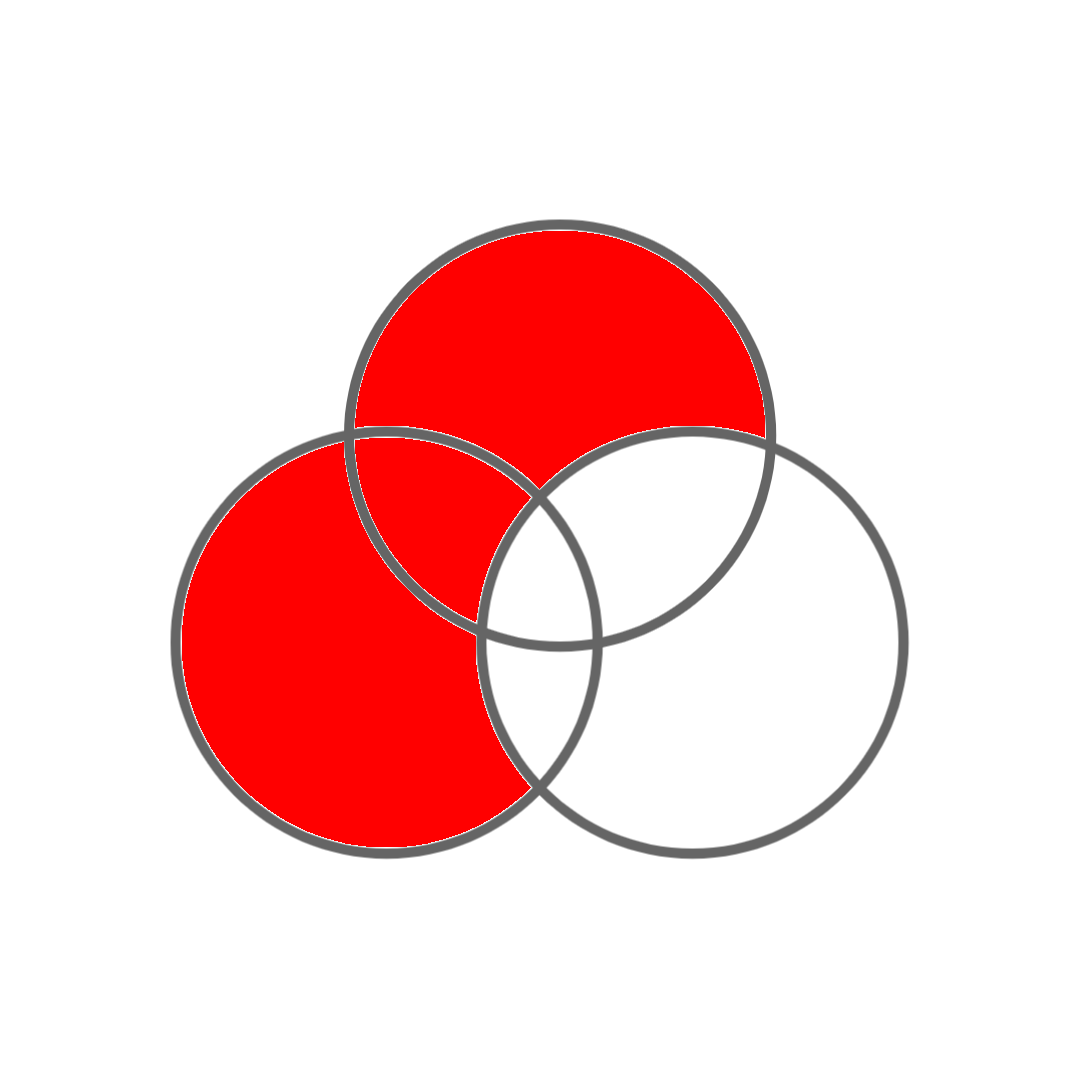
\includegraphics[scale=0.20]{images/vd_3.png}
\end{enumerate}

\noindent{\bf{50: (2 point)}}\newline
\noindent{Show that if $A$ and $B$ are finite sets, then $A\cup B$ is a finite set.}\newline
If one of the two sets is empty, then $A\cup B$ is only the non-empty set, and thus, finite.
We can move one element of the non-empty set into the empty set. This process does not change $A\cup B$ as this set contains all the elements originally in the non-empty set. We can keep moving one element from the non-empty set into the empty set until the non-empty set becomes empty. Since the sets are finite, this process will eventually swap the contents of the two sets.

\end{document}
